% This is the Amherst College LaTeX thesis template.
% See http://web.reed.edu/cis/help/latex.html for help. There are a
% great bunch of help pages there, with notes on
% getting started, bibtex, etc. Go there and read it if you're not
% already familiar with LaTeX.
%
% Any line that starts with a percent symbol is a comment.
% They won't show up in the document, and are useful for notes
% to yourself and explaining commands.
% Commenting also removes a line from the document;
% very handy for troubleshooting problems. -BTS

% As far as I know, this follows the requirements laid out in
% the 2002-2003 Senior Handbook. Ask a librarian to check the
% document before binding. -SN

%%
%% Preamble
%%
% \documentclass{<something>} must begin each LaTeX document
\documentclass[12pt,twoside]{amherstthesis}
% Packages are extensions to the basic LaTeX functions. Whatever you
% want to typeset, there is probably a package out there for it.
% Chemistry (chemtex), screenplays, you name it.
% Check out CTAN to see: http://www.ctan.org/
%%
\usepackage{graphicx,latexsym}
\usepackage{amsmath}
\usepackage{amssymb,amsthm}
\usepackage{longtable,booktabs,setspace}
\usepackage{chemarr} %% Useful for one reaction arrow, useless if you're not a chem major
\usepackage{rotating}

% Modified by CII
\usepackage[hyphens]{url}
\usepackage{hyperref}
\usepackage{lmodern}

% Added by CII (Thanks, Hadley!)
% Use ref for internal links
\renewcommand{\hyperref}[2][???]{\autoref{#1}}
\def\chapterautorefname{Chapter}
\def\sectionautorefname{Section}
\def\subsectionautorefname{Subsection}

\usepackage{caption}
\captionsetup{width=5in}

% \usepackage{times} % other fonts are available like times, bookman, charter, palatino

\title{My Comprehensive Evaluation}
\author{Kaitlyn E. Haase}
% The month and year that you submit your FINAL draft TO THE LIBRARY (May or December)
\date{February 26 2019}
\division{Statistics}
\advisor{Advisor A. Wagaman}
%If you have two advisors for some reason, you can use the following
%\altadvisor{Your Other Advisor}
%%% Remember to use the correct department!
\department{Mathematics and Statistics}
% if you're writing a thesis in an interdisciplinary major,
% uncomment the line below and change the text as appropriate.
% check the Senior Handbook if unsure.
%\thedivisionof{The Established Interdisciplinary Committee for}
% if you want the approval page to say "Approved for the Committee",
% uncomment the next line
%\approvedforthe{Committee}

% Below added by CII

%%% Copied from knitr
%% maxwidth is the original width if it's less than linewidth
%% otherwise use linewidth (to make sure the graphics do not exceed the margin)
\makeatletter
\def\maxwidth{ %
  \ifdim\Gin@nat@width>\linewidth
    \linewidth
  \else
    \Gin@nat@width
  \fi
}
\makeatother

\renewcommand{\contentsname}{Table of Contents}

\setlength{\parskip}{0pt}

\providecommand{\tightlist}{%
  \setlength{\itemsep}{0pt}\setlength{\parskip}{0pt}}

\Acknowledgements{
I want to thank my family.
}

\Dedication{

}

\Preface{

}

\Abstract{
In recent years, the amount of geographic data has increased immensely.
With new technology, the accuracy and complexity of data has also
improved. This has provoked statisticians to create techniques to best
analyze and draw conclusions from this new-found data. Earlier
techniques of spatial data were not equipped to handle the complexity
and quantity of the data. This project first explores how and why we
analyze data based on geographic information. Next, I will explain some
of the newer spatial data algorithms, including PAM (Partitioning Around
Medoids), CLARA (Clustering LARge Applications), and CLARANS (Clustering
Large Applications based on RANdomized Search). Example data will be
used to demonstrate CLARA, and the project will conclude a model to
predict cluster.
}


%%
%% End Preamble
%%
%

\begin{document}

      \maketitle
  
  \frontmatter % this stuff will be roman-numbered
  \pagestyle{empty} % this removes page numbers from the frontmatter

      \begin{acknowledgements}
      I want to thank my family.
    \end{acknowledgements}
  
  
  % Add table of abbreviations?

      \hypersetup{linkcolor=black}
    \setcounter{tocdepth}{2}
    \tableofcontents
  
      \listoftables
  
      \listoffigures
  
      \begin{abstract}
      In recent years, the amount of geographic data has increased immensely.
      With new technology, the accuracy and complexity of data has also
      improved. This has provoked statisticians to create techniques to best
      analyze and draw conclusions from this new-found data. Earlier
      techniques of spatial data were not equipped to handle the complexity
      and quantity of the data. This project first explores how and why we
      analyze data based on geographic information. Next, I will explain some
      of the newer spatial data algorithms, including PAM (Partitioning Around
      Medoids), CLARA (Clustering LARge Applications), and CLARANS (Clustering
      Large Applications based on RANdomized Search). Example data will be
      used to demonstrate CLARA, and the project will conclude a model to
      predict cluster.
    \end{abstract}
  
  
  \mainmatter % here the regular arabic numbering starts
  \pagestyle{fancyplain} % turns page numbering back on

  In recent years, the amount of geographic data has increased immensely.
  With new technology, the accuracy and complexity of data has also
  improved. This has provoked statisticians to create techniques to best
  analyze and draw conclusions from this new-found data. Earlier
  techniques of spatial data were not equipped to handle the complexity
  and quantity of the data. This project first explores how and why we
  analyze data based on geographic information. Next, I will explain some
  of the newer spatial data algorithms, including PAM (Partitioning Around
  Medoids), CLARA (Clustering LARge Applications), and CLARANS (Clustering
  Large Applications based on RANdomized Search). Example data will be
  used to demonstrate CLARA, and the project will conclude a model to
  predict cluster.
  
  \onehalfspacing
  
  \chapter*{Introduction}\label{introduction}
  \addcontentsline{toc}{chapter}{Introduction}
  
  As mentioned in the abstract, we have much more spatial data than we
  have had in the past. Spatial data analysis is analyzing data based on
  topological, geometric, and geographic information. Spatial data may
  include latitude and longitude, zip code, or street address.
  
  \section{Why Analyze Spatial Data?}\label{why-analyze-spatial-data}
  
  We are interested in analyzing spatial data for many reasons, one being
  because there is so much of it available. Investigating spatial data can
  help us find dissimilarities and similarities among objects. This can
  aid us in allocating resources to areas that need them most, discovering
  changes over time, and categorizing new objects.
  
  \section{Analyzing Spatial Data
  Algorithms}\label{analyzing-spatial-data-algorithms}
  
  There are many algorithms out there that handle spatial data; most
  algorithms are focused around clustering. To get a glimpse of the number
  of algorithms and strategies to analyze spatial data, the chart below
  provides some examples.
  
  \begin{Shaded}
  \begin{Highlighting}[]
  \KeywordTok{label}\NormalTok{(}\DataTypeTok{path =} \StringTok{"clustering_methods.png"}\NormalTok{, }
        \DataTypeTok{caption =} \StringTok{"Clustering Methods"}\NormalTok{, }
        \DataTypeTok{label =} \StringTok{"Clustering"}\NormalTok{, }\DataTypeTok{type =} \StringTok{"figure"}\NormalTok{, }\DataTypeTok{scale=} \FloatTok{0.5}\NormalTok{)}
  \end{Highlighting}
  \end{Shaded}
  
  \begin{figure}[htbp]
  \centering
  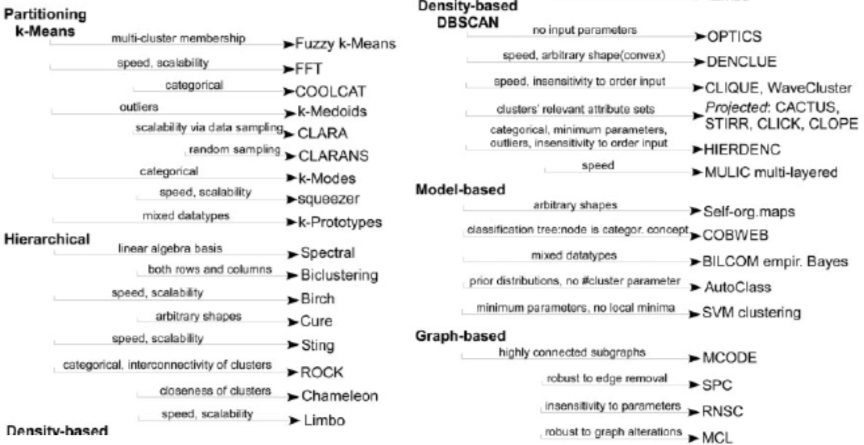
\includegraphics[scale = 0.5,angle = 0]{clustering_methods.png}
  \caption[Clustering Methods]{\normalsize{Clustering Methods}}
  \label{fig:Clustering}
  \end{figure}
  
  As noted, the methods are aimed around clustering, which we will further
  explore in the next section.
  
  \subsection{Clustering}\label{clustering}
  
  Clustering organizes a set of data items into groups so that items in
  the same group are similar to each other and different from those in
  other groups {[}Rec 1{]}. Clustering is helpful in finding patterns and
  similarities/differences between data points and groups; however it can
  be quite subjective. It is up to the statistician to determine how many
  clusters are appropriate for the data, as well as the cut off for what
  is considered ``dissimilar'' or ``similar''. Additionally, the
  statistician must choose which clustering algorithm is best to
  use\ldots{} This will be discussed in more detail later on in the
  project.
  
  \chapter{How to Cluster}\label{rmd-basics}
  
  There are many factors to consider when choosing a clustering algorithm,
  such as the application of the problem (what do you want to find out
  about this data?), quality vs speed trade off (the size of the data
  plays a role), characteristics of the data (i.e.~numeric distance
  measures), dimensionality (typically as dimension increases the time it
  takes to run the method increases and quality of the data clusters
  decrease), and outliers (some methods are very sensitive to outliers)
  {[}Rec 2{]}.
  
  \section{Types of Clustering:
  Partitioning}\label{types-of-clustering-partitioning}
  
  There are four main types of clustering: hierarchical, partitioning,
  density-based, and methods-based. Next, I'll dive into the partitioning
  clustering technique.
  
  Partitioning cluster methods divide a set of data items into a number of
  non-overlapping clusters. A data item is typically assigned to a cluster
  based on a proximity or dissimilarity measure {[}Rec 2, p.~405{]}.
  
  Usually, there is a data set with \emph{n} observations and the goal is
  to divide the data points into \emph{K} clusters so that an objective
  function is optimized.
  
  The most common objective function is the sum of squared errors (SSE),
  where \(c_k\) is the centroid or medoid of the cluster \(C_k\).
  
  \[SSE(C)= \sum_{k=1}^K \sum_{x_{i}C_{k}} ||{x_i}- c_k||^2\]
  
  Partitioning clustering algorithms classify the data into K groups by
  satisfying both that each group has at least one data point, and that
  each data point belongs to exactly one group. {[}Rec 5, p.~18{]}.
  
  \section{\texorpdfstring{Methods to Create Clusters:
  \emph{K}-Medoids}{Methods to Create Clusters: K-Medoids}}\label{methods-to-create-clusters-k-medoids}
  
  There are many ways to create clusters. The most basic method is the
  \emph{K}-means algorithm, which was developed by MacQueen in 1967 {[}Rec
  5, p.~18{]}. In response to \emph{K}-means being very sensitive to
  outliers, the \emph{K}-medoid algorithm was created in 1987 {[}Rec 5,
  p.~19{]}. Both partitioning methods use iterative processes to find
  \emph{K} clusters; however, they use different ways to represent these
  clusters.
  
  \subsection{\texorpdfstring{\emph{K}-Means}{K-Means}}\label{k-means}
  
  \emph{K}-means algorithm represents its n observations in \emph{k}
  groups, with the center of the groups being the mean/average
  observation. The goal of the algorithm is to find k centroids, one for
  each cluster. In order to do this, we must minimize an \emph{objective
  function}, which is the squared error function for \emph{k} means. The
  objective function is:
  \[O= \sum_{j=1}^k \sum_{i=1}^j ||{{X_i^{(j)}- C_j}}||^2\]
  
  Where \(|{{X_i^{(j)}- C_j}}|\) is an indicator of the distance of the
  data points from their cluster centers.
  
  The steps of the algorithm are as follows:
  
  \begin{enumerate}
  \def\labelenumi{\arabic{enumi}.}
  \tightlist
  \item
    Choose K points in the space to represent the centroid. This works
    best if they are chosen to be far apart from each other.
  \item
    Assign each object in the data set to the cluster with the closest
    centroid.
  \item
    When all of the clusters have been made, recalculate the positions of
    the K centroids.
  \item
    Repeat steps 2 and 3 until the centroids no longer move.
  \end{enumerate}
  
  This algorithm always terminates; however, it is sensitive both to
  outliers and to the initial randomly selected K cluster centers.
  Therefore, the algorithm should be run multiple times to reduce the
  effects from this sensitivity.
  
  {[}Rec 5, p.~18{]}
  
  In order to determine how well \_K\_means worked, we use the within
  cluster sum-of-squares to determine the compactness/``goodness'' of the
  clustering (and we want it as small as possible).
  
  We calculate the WSS by the following equation:
  
  \[WSS = \sum_{k=1}^k \sum_{x_i=C_k} ({{x_i- mu_k}})^2\] Where \(x_i\) is
  a data point in cluster \(C_k\) and \(mu_k\) is the mean value assigned
  to the cluster \(C_k\). {[}Rec 7{]}.
  
  \subsection{\texorpdfstring{\emph{K}
  Medoids}{K Medoids}}\label{k-medoids}
  
  On the contrary, instead of taking the mean value of the objects in a
  cluster, the k-medoid method uses the most centrally located object in a
  cluster to be the cluster center {[}Rec 2{]}. This causes the method to
  be less sensitive to outliers, but also requires more time to run.
  
  Steps for K-medoids: 1. Initial guess for centers \(C_1\),
  \(C_2\),\ldots{} \(C_k\) (i.e.~randomly select k points from \(X_1\),
  \(X_2\),\ldots{} \(X_n\)) 2. Minimize over C: for each i= 1, 2,\ldots{}
  n, find the cluster center \(C_k\) closest to Xi and let C(i)=k. 3.
  Minimize over \(C_1\), \(C_2\),\ldots{} \(C_k\): for each k=1,\ldots{}
  K, \(C_k = X_k^*\), the medoid of points in cluster k. ie, the point Xi
  in the cluster k that minimizes \[\sum  _{c(j)=k} ||{{X_j- X_i}}||^2\]
  
  Basically, \_K\_means and \_K\_medoids follow very similar algorithms;
  however, \_K\_medoids uses the most centrally located object (medoid) in
  a cluster to be the cluster center. This causes there to only be at most
  one center changed for each iteration (makes the algorithm run slower).
  {[}rec 2, p.~6{]}.
  
  \section{\texorpdfstring{How to Choose
  \emph{K}}{How to Choose K}}\label{how-to-choose-k}
  
  Now that we've discussed different kinds of \_K\_means and \_K\_medoids
  partitioning methods, we know how to find \emph{K} clusters of data
  points; but how do we determine what \emph{K} is?
  
  Well, there are many ways to choose \emph{k}, which is why these methods
  are so subjective.
  
  I will describe two of the many ways to determine \emph{K}, both of
  which use visuals to determine what value of \emph{k} is appropriate for
  the data. The elbow method and silhouette method are common ways to find
  \emph{K} when using the \emph{K} means and \emph{K} medoids algorithms.
  
  \subsection{Elbow Method}\label{elbow-method}
  
  To start, the elbow method looks at the total within-cluster sum of
  squares (WSS) and determines when there are enough clusters so that the
  next cluster does not improve the total WSS very much. This would be the
  appropriate \emph{K} to choose.
  
  The steps for this algorithm are as follows:
  
  \begin{enumerate}
  \def\labelenumi{\arabic{enumi}.}
  \tightlist
  \item
    Compute the clustering algorithm (i.e. \_k\_medoids method) for
    different values of \emph{k} (i.e. \emph{k} from 1 to 10).
  \item
    For each \emph{k}, calculate the total WSS. WSS can be calculated as:
  \end{enumerate}
  
  \[WSS= \sum_{i=1}^k \sum_{x_i = C_k} ||{{x_i- c_k}}||^2\] Where \(x_i\)
  is a data point in cluster \(C_k\) and \(c_k\) is the medoid assigned to
  the cluster \(C_k\). {[}Rec 7{]}.
  
  \begin{enumerate}
  \def\labelenumi{\arabic{enumi}.}
  \setcounter{enumi}{2}
  \tightlist
  \item
    Plot the curve of the total WSSs according to the number of clusters
    (k).
  \item
    The location of the bend in the plot is generally considered an
    indicator for the appropriate number of clusters.
  \end{enumerate}
  
  There will be an example of this method used in Chapter 3.
  
  \subsection{Silhouette Method}\label{silhouette-method}
  
  The Silhouette Method focuses on the quality of clustering. A high
  average silhouette width indicates a good clustering (how well each
  object lies within its cluster).
  
  The steps of the Silhouette Algorithm are:
  
  \begin{enumerate}
  \def\labelenumi{\arabic{enumi}.}
  \tightlist
  \item
    Compute clustering algorithm for different values of k (i.e.~k from 1
    to 10).
  \item
    For each k, calculate the average silhouette of observations. There is
    a silhouette method in R that can calculate this for us\ldots{}
  \item
    Plot the curve of the average silhouettes according to the number of
    clusters (k).
  \item
    The location of the maximum is considered the appropriate number of
    clusters.
  \end{enumerate}
  
  There will also be an example of this method used in Chapter 3.
  --\textgreater{} datanovia website
  
  \chapter{Clustering Methods Continued}\label{typeset-equ}
  
  \section{PAM}\label{pam}
  
  Partitioning Around Medoids (PAM) is the most commonly used type of
  k-medoid clustering (Kaufmann \& Rousseeuw, 1987).
  
  It iterates through all the k cluster centers and tries to replace the
  center with one of the other objects (n-k possibilities) {[}Rec 2{]}.
  For a replacement to occur, the squared error function must decrease (if
  it does not decrease, there is no replacement). The algorithm eventually
  terminates with a local optimum.
  
  The squared error function calculates the average dissimilarity
  
  The total complexity of PAM in one iteration is \[O(k(n-k)^2)\] (O= each
  non-medoid data point, \emph{k}= \# of cluster centers, \[(n-k)\]
  objects to compare to, and \[(n-k)\] operations for calculating E). This
  makes for a costly computation when n is large. The algorithm works best
  when n= 100 and \emph{k}=5.
  
  Explanation of PAM, REC 6, P. 146--\textgreater{} 4 cases, and algorithm
  Rec 6 bibliography (Ng \& Han, 2000)
  
  \section{CLARA}\label{clara}
  
  Because PAM does not scale well to large data sets, Clustering LARge
  Applications (CLARA) was developed to deal with larger data sets
  (Kaufmann \& Rousseeuw, 1990).
  
  CLARA is a sampling based method, meaning a sample of the data is used
  to represent the entire data set. Medoids are chosen from this sample
  data using PAM and then ``the average dissimilarity is computed using
  the whole dataset'' (**don't know what ``average dissimilarity'' means
  or how it is calculated). If a new set of medoids gives a lower
  dissimilarity than a previous best solution, then the best solution is
  replaced with a new set of medoids {[}Rec 2, p.~7{]}.
  
  Experiments indicate that 5 samples of size 40+ 2 \emph{k} give
  satisfactory results {[}Rec 6, p.~146{]}.
  
  The steps for the algorithm are as follows: 1. For i= 1 to 5, repeat the
  following steps: 2. Draw a sample of 40+ 2 \emph{k} objects from the
  entire data set, and use PAM to find \emph{k} medoids of the sample. 3.
  For each object \(O_j\) in the entire data set, determine which of the
  \emph{k} medoids are most similar to \(O_j\). 4. Calculate the average
  dissimilarity of the clustering obtained in the previous step. If this
  value is less than the current minimum, use this value as the current
  minimum, and retain the \emph{k} meoids found in Step 2 as the best
  medoids obtained so far. 5. Return to Step 1 to start the next
  iteration.
  
  *PAM on samples
  
  \url{https://www.coursera.org/lecture/cluster-analysis/3-4-the-k-medoids-clustering-method-nJ0Sb}
  
  \section{CLARANS}\label{clarans}
  
  (Ng \& Han, 1994)
  
  *Randomized re-sampling, ensuring efficiency and quality
  
  \begin{Shaded}
  \begin{Highlighting}[]
  \CommentTok{#How to insert a figure, make sure amherst.png is in main directory}
  
  \KeywordTok{label}\NormalTok{(}\DataTypeTok{path =} \StringTok{"clustering_pic.png"}\NormalTok{, }
        \DataTypeTok{caption =} \StringTok{"CLARANS searching for a better solution"}\NormalTok{, }
        \DataTypeTok{label =} \StringTok{"CLARANS"}\NormalTok{, }\DataTypeTok{type =} \StringTok{"figure"}\NormalTok{, }\DataTypeTok{scale=} \FloatTok{0.5}\NormalTok{)}
  \end{Highlighting}
  \end{Shaded}
  
  \begin{figure}[htbp]
  \centering
  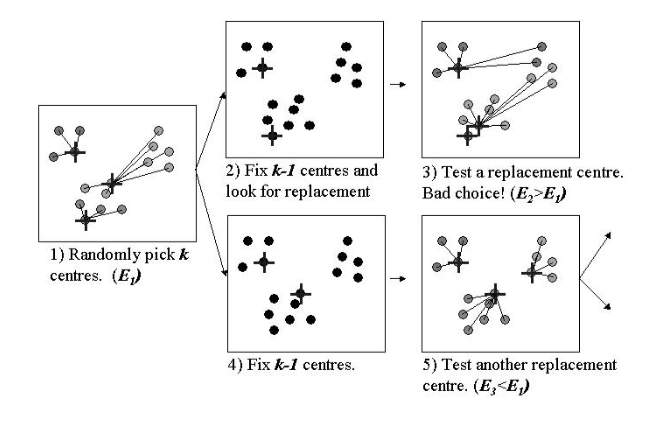
\includegraphics[scale = 0.5,angle = 0]{clustering_pic.png}
  \caption[CLARANS searching for a better solution]{\normalsize{CLARANS searching for a better solution}}
  \label{fig:CLARANS}
  \end{figure}
  
  \chapter{Example}\label{typeset-equ}
  
  \begin{Shaded}
  \begin{Highlighting}[]
  \CommentTok{#loading in packages}
  \KeywordTok{library}\NormalTok{(readr)}
  \KeywordTok{library}\NormalTok{(factoextra)}
  \end{Highlighting}
  \end{Shaded}
  
  \begin{verbatim}
  Welcome! Related Books: `Practical Guide To Cluster Analysis in R` at https://goo.gl/13EFCZ
  \end{verbatim}
  
  \begin{Shaded}
  \begin{Highlighting}[]
  \KeywordTok{library}\NormalTok{(NbClust)}
  \KeywordTok{library}\NormalTok{(ggplot2)}
  \KeywordTok{library}\NormalTok{(cluster)}
  \KeywordTok{library}\NormalTok{(GGally)}
  \end{Highlighting}
  \end{Shaded}
  
  \begin{verbatim}
  
  Attaching package: 'GGally'
  \end{verbatim}
  
  \begin{verbatim}
  The following object is masked from 'package:dplyr':
  
      nasa
  \end{verbatim}
  
  \section{Exploring the Data}\label{exploring-the-data}
  
  In this example, I will further explore the data from my Stat 495 final
  project. The data is from DataUSA, which uses public US Government data
  to analyze and visualize relationships. In the project, we decided to
  use data from 2016 because of size restrictions. The data contains
  spatial information, quantitative, and a few categorical variables.
  
  There is demographic information as well as variables that are
  indicators of health status. The health status variables include: poor
  to fair health (the percentage of adults reporting fair or poor health
  (age-adjusted)), poor physical health days (average number of physically
  unhealthy days reported in the past 30 days (age-adjusted)), physical
  inactivity (the percentage of adults aged 20 and over reporting no
  leisure-time physical inactivity), and adult obesity (the percentage of
  adults to report a BMI of greater than or equal to 30). In interpreting
  the health indicator variables, the higher the values for these
  variables, the less healthy a person is.
  
  For our Stat 495 project, we used mapping techniques to visualize and
  analyze the data. We were unable to draw many conclusions from the map,
  which is why I am interested in analyzing the data through clustering.
  Since clustering utilizes spatial information, it may be helpful in
  finding patterns in the data.
  
  My research question is to see whether there are clusters of people with
  exceptionally good or exceptionally poor health. This information could
  lead to further insights into what environmental or other factors are
  impacting peoples' health.
  
  I plan to use the CLARA method, since I have more than 100 observations.
  The data set in fact has over 60,000 observations, so I will need to
  sample about 1000 observations in order to produce the best results
  using CLARA.
  
  My first step is to import the data.
  
  \begin{Shaded}
  \begin{Highlighting}[]
  \CommentTok{#using data from final stat 495 project}
  \CommentTok{#library(readr)}
  \NormalTok{data_subset <-}\StringTok{ }\KeywordTok{read_csv}\NormalTok{(}\StringTok{"CopyOfdata_subset.csv"}\NormalTok{)}
  \end{Highlighting}
  \end{Shaded}
  
  \begin{verbatim}
  Parsed with column specification:
  cols(
    .default = col_double(),
    geo_name = col_character(),
    geo = col_character(),
    zip = col_character(),
    TRI.ID = col_character(),
    County.x = col_character(),
    County.y = col_character()
  )
  \end{verbatim}
  
  \begin{verbatim}
  See spec(...) for full column specifications.
  \end{verbatim}
  
  Next, I will take a random sample of 1000 observations. I assume the
  sample is representative of the data set because n=1000.
  
  \begin{Shaded}
  \begin{Highlighting}[]
  \KeywordTok{set.seed}\NormalTok{(}\DecValTok{1}\NormalTok{)}
  \CommentTok{#getting a sample of 1000 observations}
  \NormalTok{mysample <-}\StringTok{ }\NormalTok{data_subset[}\KeywordTok{sample}\NormalTok{(}\DecValTok{1}\OperatorTok{:}\KeywordTok{nrow}\NormalTok{(data_subset), }\DecValTok{1000}\NormalTok{,}
     \DataTypeTok{replace=}\OtherTok{FALSE}\NormalTok{),]}
  \end{Highlighting}
  \end{Shaded}
  
  The data set I imported has 64 variables, which are too many for this
  example. Since my research question is focused around peoples' health, I
  will only include the health indicator variables and the latitude and
  longitude of the data (spatial information).
  
  \begin{Shaded}
  \begin{Highlighting}[]
  \CommentTok{#only keeping the variables I want to look at}
  \NormalTok{myvars <-}\StringTok{ }\KeywordTok{c}\NormalTok{(}\StringTok{"Latitude_tri"}\NormalTok{, }\StringTok{"Longitude_tri"}\NormalTok{, }\StringTok{"poor_or_fair_health"}\NormalTok{, }\StringTok{"poor_physical_health_days"}\NormalTok{, }\StringTok{"physical_inactivity"}\NormalTok{, }\StringTok{"adult_obesity"}\NormalTok{)}
  \NormalTok{smallsample <-}\StringTok{ }\NormalTok{mysample[myvars]}
  \end{Highlighting}
  \end{Shaded}
  
  The data is now ready to apply CLARA.
  
  \section{Applying CLARA}\label{applying-clara}
  
  Step 1: Determining \emph{k}.
  
  One of the major steps in clustering algorithms is determining how many
  \emph{k} clusters is appropriate. In Chapter 1, I explained the Elbow
  and Silhouette methods of determining \emph{k}. I will perform both
  methods on this data to start.
  
  \begin{Shaded}
  \begin{Highlighting}[]
  \CommentTok{#finding k with project data, using Elbow Method}
  \CommentTok{#pkgs <- c("factoextra",  "NbClust")}
  \CommentTok{#install.packages(pkgs)}
  
  \CommentTok{#library(factoextra)}
  \CommentTok{#library(NbClust)}
  \CommentTok{#library(ggplot2)}
  \CommentTok{#first I must omit any of the missing data, so that the functions can run}
  \NormalTok{new<-}\StringTok{ }\KeywordTok{na.omit}\NormalTok{(smallsample)}
  \CommentTok{# Elbow method}
  \CommentTok{#fviz_nbclust(new, kmeans, method = "wss") +}
   \CommentTok{#   geom_vline(xintercept = 4, linetype = 2)+}
    \CommentTok{#labs(subtitle = "Elbow method")}
  
  \KeywordTok{fviz_nbclust}\NormalTok{(new, kmeans, }\DataTypeTok{method =} \StringTok{"wss"}\NormalTok{) }\OperatorTok{+}
  \StringTok{    }\KeywordTok{geom_vline}\NormalTok{(}\DataTypeTok{xintercept =} \DecValTok{4}\NormalTok{, }\DataTypeTok{linetype =} \DecValTok{2}\NormalTok{)}\OperatorTok{+}
  \StringTok{  }\KeywordTok{labs}\NormalTok{(}\DataTypeTok{subtitle =} \StringTok{"Elbow method"}\NormalTok{)}
  \end{Highlighting}
  \end{Shaded}
  
  \begin{center}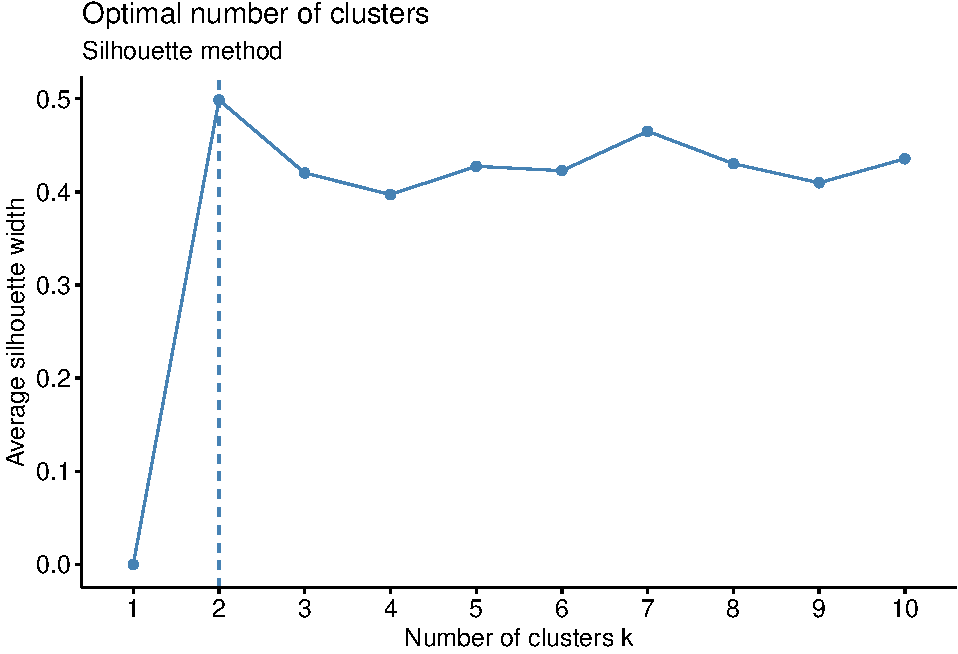
\includegraphics{Comps_Proj_files/figure-latex/unnamed-chunk-5-1} \end{center}
  
  \begin{Shaded}
  \begin{Highlighting}[]
  \KeywordTok{fviz_nbclust}\NormalTok{(new, kmeans, }\DataTypeTok{method =} \StringTok{"silhouette"}\NormalTok{) }\OperatorTok{+}
  \StringTok{  }\KeywordTok{labs}\NormalTok{(}\DataTypeTok{subtitle =} \StringTok{"Silhouette method"}\NormalTok{)}
  \end{Highlighting}
  \end{Shaded}
  
  \begin{center}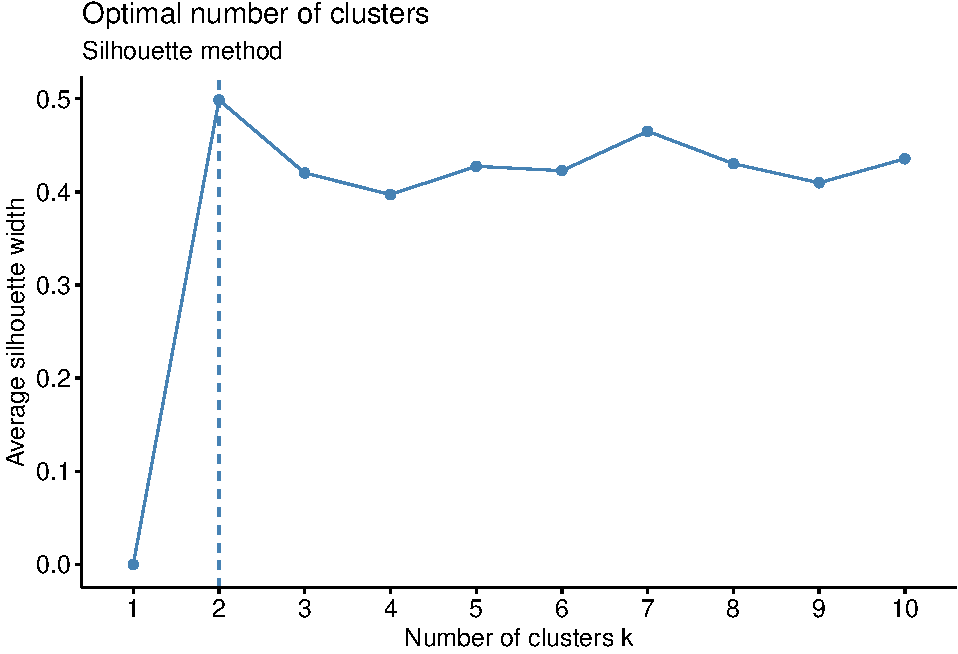
\includegraphics{Comps_Proj_files/figure-latex/unnamed-chunk-5-2} \end{center}
  
  According to the Elbow method, \emph{k} should be 4 (where the elbow is
  in the graph). According to the Silhouette method, \emph{k} should be 2
  (the maximum point in the graph). Since there is variation in values of
  \emph{k} for these methods I will take the average of the two to
  determine \emph{k}.
  
  Step 2: Run CLARA function
  
  Next, I will run the CLARA algorithm on the data, using the criteria of
  \emph{k}=3.
  
  \begin{Shaded}
  \begin{Highlighting}[]
  \CommentTok{#library(cluster)}
  \NormalTok{## run CLARA}
  \NormalTok{clarasamp <-}\StringTok{ }\KeywordTok{clara}\NormalTok{(new[}\DecValTok{1}\OperatorTok{:}\DecValTok{6}\NormalTok{], }\DecValTok{3}\NormalTok{)}
  \end{Highlighting}
  \end{Shaded}
  
  \begin{Shaded}
  \begin{Highlighting}[]
  \NormalTok{## print components of clara}
  \KeywordTok{print}\NormalTok{(clarasamp)}
  \end{Highlighting}
  \end{Shaded}
  
  \begin{verbatim}
  Call:    clara(x = new[1:6], k = 3) 
  Medoids:
       Latitude_tri Longitude_tri poor_or_fair_health
  [1,]      39.3265      -84.4388               0.155
  [2,]      40.3973      -75.9357               0.165
  [3,]      36.1336      -96.1039               0.196
       poor_physical_health_days physical_inactivity adult_obesity
  [1,]                       3.7               0.232         0.289
  [2,]                       3.7               0.245         0.308
  [3,]                       4.6               0.353         0.355
  Objective function:  5.659219
  Clustering vector:   int [1:925] 1 2 1 3 1 3 1 1 1 1 1 3 1 2 1 3 1 3 ...
  Cluster sizes:           457 205 263 
  Best sample:
   [1]   5  24  86 139 149 175 177 192 208 224 242 285 306 316 333 353 361
  [18] 370 389 400 404 410 429 468 471 489 502 506 567 593 679 691 703 719
  [35] 726 741 780 800 811 815 818 877 882 883 902 918
  
  Available components:
   [1] "sample"     "medoids"    "i.med"      "clustering" "objective" 
   [6] "clusinfo"   "diss"       "call"       "silinfo"    "data"      
  \end{verbatim}
  
  This output tells us a lot about the results of the clustering. To
  start, the information from the Medoids section show that cluster 3
  contains people with the worst health, in comparison to cluster 1 and 2.
  For example, cluster 1 and 2 average 3.7 poor\_physical\_health\_days,
  while cluster 3 averages 4.6. This difference was seen in all four
  health indicator variables.
  
  The cluster sizes are also noted. There are 457 observations in cluster
  1, 205 in cluster 2, and 263 in cluster 3.
  
  \begin{Shaded}
  \begin{Highlighting}[]
  \CommentTok{#more output from CLARA}
  
  \CommentTok{#cluster number for each observation}
  \KeywordTok{print}\NormalTok{(clarasamp}\OperatorTok{$}\NormalTok{cluster)}
  \end{Highlighting}
  \end{Shaded}
  
  \begin{verbatim}
    [1] 1 2 1 3 1 3 1 1 1 1 1 3 1 2 1 3 1 3 3 2 1 3 2 1 1 1 3 2 2 1 1 2 3 1 3
   [36] 2 1 1 3 3 1 1 1 1 1 1 1 1 1 2 1 1 1 1 1 1 1 3 1 1 1 1 2 2 3 3 1 2 1 3
   [71] 1 1 3 3 1 3 1 3 1 2 1 2 3 1 1 3 1 2 3 3 3 3 1 1 3 3 3 1 2 2 1 2 3 3 1
  [106] 1 1 3 3 3 1 3 3 3 2 1 2 3 2 3 2 2 1 3 1 2 1 1 1 3 2 3 1 2 1 1 2 1 3 3
  [141] 1 2 1 1 1 1 2 1 1 2 2 1 1 3 3 1 3 1 3 1 3 1 1 2 1 3 1 3 3 1 1 3 1 3 3
  [176] 1 3 1 2 3 2 1 2 1 1 2 1 1 3 1 1 3 2 1 2 3 3 2 1 1 1 2 1 3 2 1 2 1 1 1
  [211] 1 1 1 2 1 3 3 2 3 3 1 1 3 2 1 1 3 3 3 2 2 1 1 1 3 3 1 1 1 1 1 2 1 2 3
  [246] 2 1 1 1 1 1 3 3 2 1 1 2 1 1 2 1 1 1 3 2 3 2 3 2 2 3 2 2 3 1 1 3 2 1 3
  [281] 2 1 1 3 1 1 3 1 2 2 3 1 1 3 1 2 1 1 1 1 1 3 1 1 1 1 3 3 1 3 1 1 3 1 1
  [316] 3 1 2 1 1 1 3 2 3 1 1 3 1 1 3 2 1 1 1 3 1 2 1 2 2 1 3 1 1 3 3 3 3 1 1
  [351] 1 1 1 1 1 3 1 3 2 1 1 3 3 1 2 2 3 1 2 3 1 3 3 2 2 2 1 1 3 2 3 3 3 1 1
  [386] 1 1 2 1 3 1 1 2 1 2 2 1 3 3 2 1 3 2 2 1 1 1 1 1 1 3 1 1 1 1 1 2 1 3 1
  [421] 3 3 2 3 1 2 1 3 2 1 1 2 1 3 3 1 1 3 1 2 1 1 1 3 1 2 1 1 2 1 3 1 1 2 3
  [456] 1 1 2 1 1 1 2 1 1 3 3 1 1 3 3 1 1 3 1 3 1 1 1 1 3 3 2 1 1 1 1 2 2 3 1
  [491] 2 3 1 3 3 1 2 2 2 2 1 2 2 3 1 1 2 3 2 1 1 2 3 2 3 3 2 2 2 1 2 1 3 2 3
  [526] 3 3 1 3 1 1 2 2 2 1 3 2 1 1 1 3 3 1 1 3 1 1 2 3 1 2 1 3 1 1 3 2 3 3 3
  [561] 1 2 1 2 1 3 2 3 1 3 1 1 3 3 2 1 1 3 2 2 1 1 2 1 2 1 1 1 1 1 2 1 3 3 1
  [596] 3 1 2 2 1 3 2 3 3 1 3 1 1 1 3 3 1 2 1 1 3 3 2 1 2 3 2 1 2 3 1 1 2 1 2
  [631] 1 1 3 3 1 2 3 1 1 3 1 3 3 1 1 1 2 2 3 2 1 1 1 2 1 1 1 2 3 1 3 1 1 3 1
  [666] 1 1 1 3 1 2 1 3 1 1 1 1 1 2 2 3 1 2 1 2 2 1 1 2 2 3 2 1 1 1 2 1 3 3 1
  [701] 1 1 1 3 2 1 3 1 1 2 3 3 1 1 1 3 3 1 1 1 1 3 1 1 2 3 2 3 1 1 1 3 1 1 3
  [736] 1 2 1 2 3 2 2 2 1 3 3 3 1 1 1 2 3 3 3 1 3 3 2 1 2 3 3 1 2 3 2 1 1 3 1
  [771] 2 1 1 1 3 1 3 1 1 1 3 1 1 3 1 2 1 1 3 1 3 1 1 1 1 3 2 2 2 3 1 3 3 1 1
  [806] 1 3 1 1 1 2 1 1 1 2 2 2 1 1 2 1 3 3 3 3 1 3 2 3 2 1 2 1 1 1 3 2 1 1 3
  [841] 2 2 2 2 2 1 3 1 2 1 2 3 3 3 1 1 3 1 1 1 1 1 2 3 3 2 3 1 2 1 1 1 1 2 1
  [876] 1 3 1 1 1 3 3 1 1 1 1 1 1 3 1 1 3 1 3 1 3 2 2 2 3 1 2 2 2 1 1 3 1 2 1
  [911] 3 1 3 2 3 3 1 1 2 1 3 1 1 3 1
  \end{verbatim}
  
  \begin{Shaded}
  \begin{Highlighting}[]
  \CommentTok{#silhouette width for each cluster}
  \KeywordTok{print}\NormalTok{(clarasamp}\OperatorTok{$}\NormalTok{silinfo)}
  \end{Highlighting}
  \end{Shaded}
  
  \begin{verbatim}
  $widths
      cluster neighbor   sil_width
  703       1        2  0.59850204
  780       1        2  0.59563931
  208       1        2  0.58522416
  149       1        2  0.55721957
  471       1        2  0.54671717
  719       1        2  0.52773515
  818       1        2  0.52638884
  410       1        2  0.52317171
  5         1        2  0.49272339
  333       1        2  0.48262589
  361       1        2  0.46877636
  306       1        2  0.46546394
  389       1        2  0.40532336
  506       1        2  0.40333194
  468       1        2  0.35920963
  353       1        3  0.32935312
  285       1        2  0.31204760
  918       1        2  0.16440373
  24        1        2  0.13034904
  883       1        2 -0.03054377
  224       2        1  0.75049734
  679       2        1  0.74239308
  404       2        1  0.73164794
  902       2        1  0.73161340
  242       2        1  0.73125890
  400       2        1  0.73078958
  502       2        1  0.65554544
  741       2        1  0.64706730
  567       2        1  0.62730880
  811       2        1  0.46502193
  815       2        1  0.40449435
  429       2        1  0.39693747
  882       3        1  0.33188295
  139       3        1  0.31419706
  726       3        1  0.31186219
  800       3        1  0.31127063
  691       3        1  0.29040279
  370       3        1  0.28765117
  489       3        1  0.28371053
  177       3        1  0.26300486
  175       3        1  0.23220663
  86        3        1  0.06439635
  593       3        1  0.03655278
  877       3        1 -0.06313781
  192       3        1 -0.11112090
  316       3        1 -0.14469112
  
  $clus.avg.widths
  [1] 0.4221831 0.6345480 0.1720134
  
  $avg.width
  [1] 0.401444
  \end{verbatim}
  
  This information tells us even more about the CLARA output. The first
  part gives us the categorizations of each data point to its cluster. The
  second part of information gives us the average silhouette width for
  each cluster. The silhouette widths were: 0.422183 for cluster 1,
  0.634548 for cluster 2, and 0.172013 for cluster 3. The better the
  clustering is, the greater the silhouette width; so we can determine
  that cluster 2 was best compared to cluster 1 and 3.
  
  Next, I will walk through some of the visualizations given this new
  clustering information.
  
  \begin{Shaded}
  \begin{Highlighting}[]
  \NormalTok{## plot clusters}
  \KeywordTok{plot}\NormalTok{(new, }\DataTypeTok{col =}\NormalTok{ clarasamp}\OperatorTok{$}\NormalTok{cluster)}
  \NormalTok{## plot centers}
  \KeywordTok{points}\NormalTok{(clarasamp}\OperatorTok{$}\NormalTok{centers, }\DataTypeTok{col =} \DecValTok{1}\OperatorTok{:}\DecValTok{2}\NormalTok{, }\DataTypeTok{pch =} \DecValTok{8}\NormalTok{)}
  \end{Highlighting}
  \end{Shaded}
  
  \begin{center}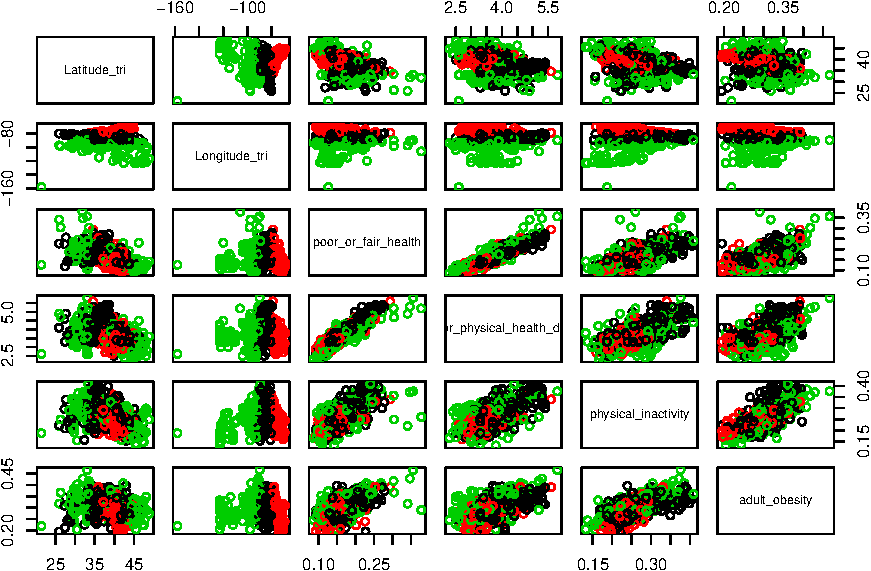
\includegraphics{Comps_Proj_files/figure-latex/unnamed-chunk-9-1} \end{center}
  
  The plot of the clusters does not look great. Aside from comparing
  longitude with the other variables, the plots have entirely overlapping
  clusters. This indicates that the CLARA method was unable to find great
  patterns in the data.
  
  Next, I will use a version of a ggplot to plot the clusters.
  
  \begin{Shaded}
  \begin{Highlighting}[]
  \CommentTok{#plotting clara}
  \NormalTok{factoextra}\OperatorTok{::}\KeywordTok{fviz_cluster}\NormalTok{(clarasamp)}
  \end{Highlighting}
  \end{Shaded}
  
  \begin{center}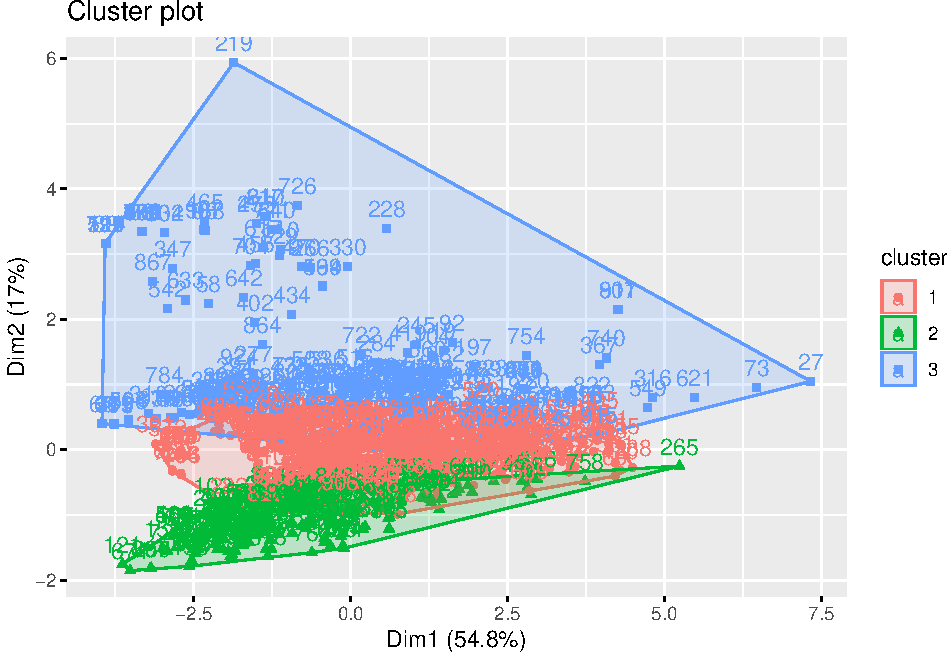
\includegraphics{Comps_Proj_files/figure-latex/unnamed-chunk-10-1} \end{center}
  
  \section{Evaluation of CLARA}\label{evaluation-of-clara}
  
  There are multiple ways to determine the effectiveness of CLARA and the
  quality of its clusters. One of the ways to internally validate the
  method, is to look at its WSS. If there is a high WSS, it is likely the
  method did not work very well.
  
  I plotted in the previous section in the Elbow method plot to determine
  the number of clusters to use. Since I decided to use \emph{k}=3
  clusters, I can now go back and calculate the WSS for the method.
  
  \begin{Shaded}
  \begin{Highlighting}[]
  \NormalTok{elbow<-}\StringTok{ }\KeywordTok{fviz_nbclust}\NormalTok{(new, kmeans, }\DataTypeTok{method =} \StringTok{"wss"}\NormalTok{) }\OperatorTok{+}
  \StringTok{    }\KeywordTok{geom_vline}\NormalTok{(}\DataTypeTok{xintercept =} \DecValTok{3}\NormalTok{, }\DataTypeTok{linetype =} \DecValTok{2}\NormalTok{)}\OperatorTok{+}
  \StringTok{  }\KeywordTok{labs}\NormalTok{(}\DataTypeTok{subtitle =} \StringTok{"Elbow method"}\NormalTok{)}
  \NormalTok{elbow}
  \end{Highlighting}
  \end{Shaded}
  
  \begin{center}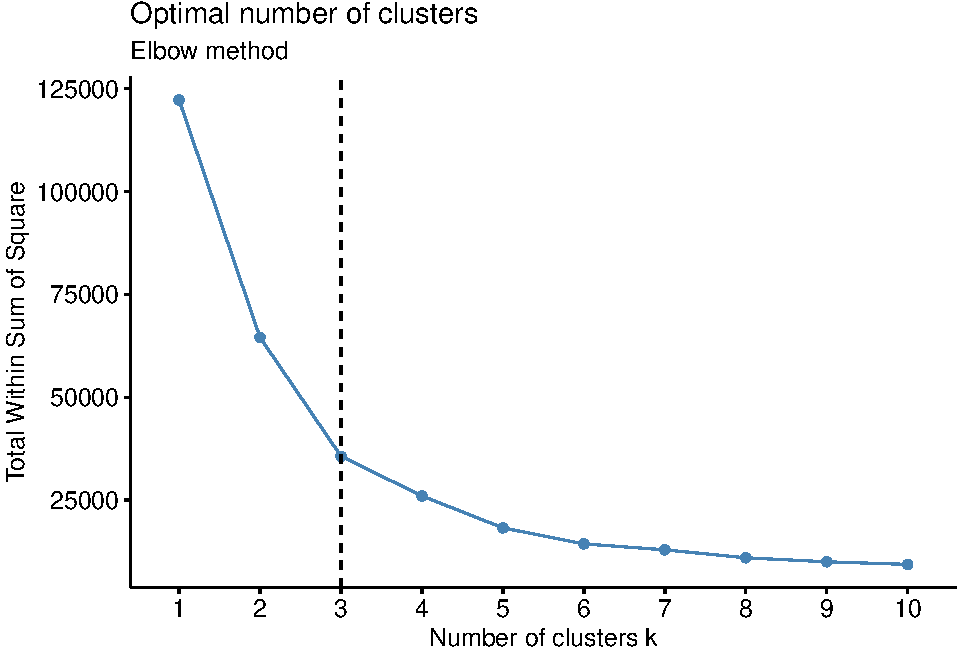
\includegraphics{Comps_Proj_files/figure-latex/unnamed-chunk-11-1} \end{center}
  
  The Elbow method when \emph{k}=3, shows a WSS to be about 30,000. This
  is very high, which is a concern when interpreting the cluster
  results\ldots{}
  
  \subsection{Model to Predict Cluster}\label{model-to-predict-cluster}
  
  The CLARA method found three clusters to group the health data. While
  the WSS value of over 30,000 indicated the clustering may not be very
  accurate or useful, I want to determine if I can predict the cluster
  number (1, 2, or 3), given the health indicators. This would be helpful
  information, say there is a new data observation and I want to
  categorize it into cluster 1, 2, or 3.
  
  To start this process, I first had to include a variable with cluster
  number (from the CLARA method) to the original sample of the data set.
  
  \begin{Shaded}
  \begin{Highlighting}[]
  \CommentTok{#adding each data point's cluster #}
  \NormalTok{cluster<-}\StringTok{ }\NormalTok{clarasamp}\OperatorTok{$}\NormalTok{clustering}
  \NormalTok{cluster_data<-}\StringTok{ }\KeywordTok{cbind}\NormalTok{(new, cluster)}
  \end{Highlighting}
  \end{Shaded}
  
  Next, I looked at possible relationships between the health indicator
  variables and cluster number. To start, I quickly looked at a
  multivariate linear regression model to predict cluster using all of the
  possible variables.
  
  \begin{Shaded}
  \begin{Highlighting}[]
  \NormalTok{kitchen_sink<-}\StringTok{ }\KeywordTok{lm}\NormalTok{(cluster}\OperatorTok{~}\NormalTok{., }\DataTypeTok{data=}\NormalTok{cluster_data)}
  \KeywordTok{summary}\NormalTok{(kitchen_sink)}
  \end{Highlighting}
  \end{Shaded}
  
  \begin{verbatim}
  
  Call:
  lm(formula = cluster ~ ., data = cluster_data)
  
  Residuals:
       Min       1Q   Median       3Q      Max 
  -2.33635 -0.62036 -0.00065  0.59937  1.48615 
  
  Coefficients:
                             Estimate Std. Error t value Pr(>|t|)    
  (Intercept)                0.383530   0.376180   1.020  0.30822    
  Latitude_tri              -0.007281   0.006479  -1.124  0.26141    
  Longitude_tri             -0.039276   0.002194 -17.905  < 2e-16 ***
  poor_or_fair_health       10.089001   1.417808   7.116 2.24e-12 ***
  poor_physical_health_days -1.081969   0.088359 -12.245  < 2e-16 ***
  physical_inactivity        1.986841   0.730739   2.719  0.00667 ** 
  adult_obesity              0.332835   0.816048   0.408  0.68347    
  ---
  Signif. codes:  0 '***' 0.001 '**' 0.01 '*' 0.05 '.' 0.1 ' ' 1
  
  Residual standard error: 0.6793 on 918 degrees of freedom
  Multiple R-squared:  0.3765,    Adjusted R-squared:  0.3724 
  F-statistic: 92.38 on 6 and 918 DF,  p-value: < 2.2e-16
  \end{verbatim}
  
  According to this model, longitude, poor\_or\_fair\_health,
  poor\_physical\_health\_days, and physical\_inactivity were strong
  predictors of cluster number. Overall, the model seemed to fit the data
  fairly well. The model had a high F-statistic and a low p-value of
  \textless{}2e-16. The adjusted R-squared value was 0.372.
  
  In analyzing this model I realized that latitude and longitude were used
  as quantitative variables instead of categorical. Since linear and
  multivariate regression predictive models only use quantitative or
  categorical variables, I realized that the latitude and longitude
  (spatial information) would not be helpful.
  
  \begin{Shaded}
  \begin{Highlighting}[]
  \CommentTok{#taking out latitude and longitude}
  \NormalTok{vars <-}\StringTok{ }\KeywordTok{names}\NormalTok{(cluster_data) }\OperatorTok\StringTok{ }\KeywordTok{c}\NormalTok{(}\StringTok{"Latitude_tri"}\NormalTok{, }\StringTok{"Longitude_tri"}\NormalTok{)}
  \NormalTok{cluster_data_new <-}\StringTok{ }\NormalTok{cluster_data[}\OperatorTok{!}\NormalTok{vars]}
  \end{Highlighting}
  \end{Shaded}
  
  I ran another kitchen sink model, with only the health variables and
  cluster information.
  
  \begin{Shaded}
  \begin{Highlighting}[]
  \NormalTok{new_kitchen_sink<-}\StringTok{ }\KeywordTok{lm}\NormalTok{(cluster}\OperatorTok{~}\NormalTok{., }\DataTypeTok{data=}\NormalTok{cluster_data_new)}
  \KeywordTok{summary}\NormalTok{(new_kitchen_sink)}
  \end{Highlighting}
  \end{Shaded}
  
  \begin{verbatim}
  
  Call:
  lm(formula = cluster ~ ., data = cluster_data_new)
  
  Residuals:
      Min      1Q  Median      3Q     Max 
  -1.4582 -0.6918 -0.1393  0.6406  2.2221 
  
  Coefficients:
                            Estimate Std. Error t value Pr(>|t|)    
  (Intercept)                 3.5366     0.2297  15.399  < 2e-16 ***
  poor_or_fair_health        13.0696     1.3988   9.343  < 2e-16 ***
  poor_physical_health_days  -1.2089     0.0964 -12.540  < 2e-16 ***
  physical_inactivity        -0.9774     0.8086  -1.209  0.22705    
  adult_obesity               2.8044     0.9247   3.033  0.00249 ** 
  ---
  Signif. codes:  0 '***' 0.001 '**' 0.01 '*' 0.05 '.' 0.1 ' ' 1
  
  Residual standard error: 0.7882 on 920 degrees of freedom
  Multiple R-squared:  0.1587,    Adjusted R-squared:  0.1551 
  F-statistic: 43.39 on 4 and 920 DF,  p-value: < 2.2e-16
  \end{verbatim}
  
  This model had three significant predictors (poor\_or\_fair\_health,
  poor\_physical\_health\_days, and adult\_obesity), a high F-statistic,
  and a low p-value of \textless{}2e-16. The model did not fit the data
  very well, and had an adjusted R-squared value of 0.155.
  
  Next, I looked at the possible correlations between cluster number and
  the health indicator variables. I predicted the healthier people (lower
  scores on the health indicator variables) would be in cluster 1, while
  the least healthy people (higher scores on health indicator variables)
  would be in cluster 3. I also predicted the health indicator variables
  would be highly correlated with each other, considering they all are
  aiding in predicting one's health.
  
  \begin{Shaded}
  \begin{Highlighting}[]
  \KeywordTok{ggpairs}\NormalTok{(cluster_data_new)}
  \end{Highlighting}
  \end{Shaded}
  
  \begin{center}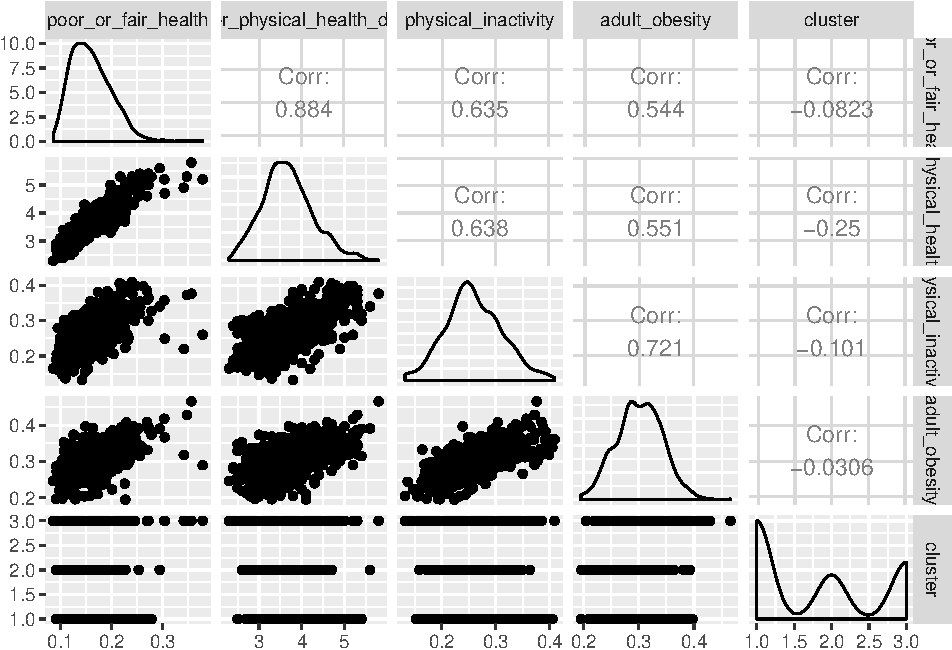
\includegraphics{Comps_Proj_files/figure-latex/unnamed-chunk-16-1} \end{center}
  
  The correlation plot shows strong positive correlations between
  poor\_or\_fair\_health, poor\_physical\_health\_days,
  physical\_inactivity, and adult\_obesity, as I had predicted. The
  highest correlation was 0.884, between poor\_physical\_health\_days and
  poor\_to\_fair\_health. All of the variables in general show bell-shaped
  curves with a relatively even shape.
  
  The plots comparing the variables to the cluster number are hard to
  interpret at first. To start, the poor\_to\_fair\_health versus cluster
  plot shows that the highest values of poor\_or\_fair\_health are in
  cluster 3. These look to be possible outliers, but regardless, it
  confirms the prediction that the unhealthy people (high health variable
  scores) are in cluster 3.
  
  The poor\_physical\_health\_days versus cluster number and
  adult\_obesity versus cluster number show a couple of observations with
  high health variable scores in cluster 3 as well. It is again unclear if
  these points are outliers or not.
  
  In general, the plots show that cluster 2 has the smallest range of
  health scores, which further confirms that cluster 2 had the highest
  quality of clustering (the largest silhouette width). In terms of
  correlation values, cluster number was shows to be sightly negatively
  correlated with poor\_physical\_health\_days, with a correlation value
  of -0.25.
  
  I had predicted the correlation to be positive, because the CLARA output
  revealed cluster 3 to have the most unhealthy people. This would mean
  the higher the health variable value, the higher the cluster number.
  Since the correlations are in fact slightly negative, I believe the
  reason for the higher health value mean score for cluster 3 was probably
  due to the outliers also shown in the plots.
  
  All of correlations between the health variables and cluster number were
  negative, indicating that the clustering was not very effective and
  instead there may be outliers impacting the original analysis of CLARA.
  
  Nevertheless, I will continue to explore possible relationships between
  health variables and cluster number. Based on the correlation plot, I
  will explore poor\_or\_fair\_health (because of the plot),
  poor\_physical\_health\_days (because of the correlation value), and
  adult\_obesity (because of the plot).
  
  I tried numerous combinations of the variables as well as interaction
  terms, because the variables are so highly correlated.
  
  \begin{Shaded}
  \begin{Highlighting}[]
  \KeywordTok{set.seed}\NormalTok{(}\DecValTok{2}\NormalTok{)}
  \CommentTok{#exploring possible relationships between health variables and cluster number}
  
  \NormalTok{fun1<-}\StringTok{ }\KeywordTok{lm}\NormalTok{(cluster}\OperatorTok{~}\StringTok{ }\NormalTok{poor_or_fair_health }\OperatorTok{+}\StringTok{ }\NormalTok{poor_physical_health_days }\OperatorTok{+}\StringTok{ }\NormalTok{adult_obesity, }\DataTypeTok{data=}\NormalTok{ cluster_data_new)}
  \CommentTok{#low adjusted R-squared (0.155), but significant predictors}
   
  \NormalTok{fun2<-}\StringTok{ }\KeywordTok{lm}\NormalTok{(cluster}\OperatorTok{~}\StringTok{ }\NormalTok{poor_or_fair_health, }\DataTypeTok{data=}\NormalTok{ cluster_data_new)}
  \NormalTok{fun3<-}\StringTok{ }\KeywordTok{lm}\NormalTok{(cluster}\OperatorTok{~}\StringTok{ }\NormalTok{poor_physical_health_days, }\DataTypeTok{data=}\NormalTok{ cluster_data_new)}
  \NormalTok{fun4<-}\StringTok{ }\KeywordTok{lm}\NormalTok{(cluster}\OperatorTok{~}\StringTok{ }\NormalTok{adult_obesity, }\DataTypeTok{data=}\NormalTok{ cluster_data_new)}
  \CommentTok{#low adjusted R-squared, highest of the 3 functions was 0.06}
  
  \NormalTok{fun5<-}\StringTok{ }\KeywordTok{lm}\NormalTok{(cluster}\OperatorTok{~}\StringTok{ }\NormalTok{poor_or_fair_health }\OperatorTok{+}\StringTok{ }\NormalTok{poor_physical_health_days }\OperatorTok{+}\StringTok{ }\NormalTok{adult_obesity }\OperatorTok{+}\StringTok{ }\NormalTok{poor_or_fair_health}\OperatorTok{:}\NormalTok{poor_physical_health_days, }\DataTypeTok{data=}\NormalTok{ cluster_data_new)}
  \CommentTok{#added an interaction, raised the adjusted R-squared to 0.165}
  
  \NormalTok{fun6<-}\StringTok{ }\KeywordTok{lm}\NormalTok{(cluster}\OperatorTok{~}\StringTok{ }\NormalTok{poor_or_fair_health }\OperatorTok{+}\StringTok{ }\NormalTok{poor_physical_health_days }\OperatorTok{+}\StringTok{ }\NormalTok{adult_obesity }\OperatorTok{+}\StringTok{ }\NormalTok{poor_physical_health_days}\OperatorTok{:}\NormalTok{adult_obesity, }\DataTypeTok{data=}\NormalTok{ cluster_data_new)}
  \CommentTok{#tried a different interaction, about the same adjusted R-squared}
  
  \NormalTok{fun7<-}\StringTok{ }\KeywordTok{lm}\NormalTok{(cluster}\OperatorTok{~}\StringTok{ }\NormalTok{poor_or_fair_health }\OperatorTok{+}\StringTok{ }\NormalTok{poor_physical_health_days }\OperatorTok{+}\StringTok{ }\NormalTok{adult_obesity }\OperatorTok{+}\StringTok{ }\NormalTok{poor_or_fair_health}\OperatorTok{:}\NormalTok{adult_obesity, }\DataTypeTok{data=}\NormalTok{ cluster_data_new)}
  \CommentTok{#last combination of an interaction, highest adjusted R-squared yet (0.175)!}
  \CommentTok{#only predictor not significant was poor_or_fair_health}
  
  \NormalTok{fun8<-}\StringTok{ }\KeywordTok{lm}\NormalTok{(cluster}\OperatorTok{~}\StringTok{  }\NormalTok{poor_physical_health_days }\OperatorTok{+}\StringTok{ }\NormalTok{adult_obesity }\OperatorTok{+}\StringTok{ }\NormalTok{poor_or_fair_health}\OperatorTok{:}\NormalTok{adult_obesity, }\DataTypeTok{data=}\NormalTok{ cluster_data_new)}
  \CommentTok{#dropped poor_or_fair_health, about the same adjusted R-squared (0.174)}
  
  \NormalTok{fun9<-}\StringTok{ }\KeywordTok{lm}\NormalTok{(cluster}\OperatorTok{~}\StringTok{ }\NormalTok{poor_physical_health_days }\OperatorTok{+}\StringTok{ }\NormalTok{adult_obesity }\OperatorTok{+}\StringTok{ }\NormalTok{poor_physical_health_days}\OperatorTok{:}\NormalTok{adult_obesity, }\DataTypeTok{data=}\NormalTok{ cluster_data_new)}
  \CommentTok{#tried a different interaction, low adjusted R-squared (0.0958)}
  
  \NormalTok{fun10<-}\StringTok{ }\KeywordTok{lm}\NormalTok{(cluster}\OperatorTok{~}\StringTok{ }\NormalTok{poor_physical_health_days }\OperatorTok{+}\StringTok{ }\NormalTok{adult_obesity }\OperatorTok{+}\StringTok{ }\NormalTok{poor_or_fair_health}\OperatorTok{:}\NormalTok{poor_physical_health_days, }\DataTypeTok{data=}\NormalTok{ cluster_data_new)}
  \CommentTok{#tried last combination of interaction, adjusted R-squared= 0.166}
  \end{Highlighting}
  \end{Shaded}
  
  Most of the model had significant predictors; however, the R-squared
  values were small; indicating that the models did not fit the data very
  well.
  
  In comparing adjusted R-squared values and the number of predictors
  used, the best model ended up being:
  
  \begin{Shaded}
  \begin{Highlighting}[]
  \KeywordTok{summary}\NormalTok{(fun8)}
  \end{Highlighting}
  \end{Shaded}
  
  \begin{verbatim}
  
  Call:
  lm(formula = cluster ~ poor_physical_health_days + adult_obesity + 
      poor_or_fair_health:adult_obesity, data = cluster_data_new)
  
  Residuals:
      Min      1Q  Median      3Q     Max 
  -1.5661 -0.6691 -0.1815  0.5856  2.2755 
  
  Coefficients:
                                    Estimate Std. Error t value Pr(>|t|)    
  (Intercept)                        5.73676    0.36071  15.904  < 2e-16 ***
  poor_physical_health_days         -1.24651    0.08954 -13.921  < 2e-16 ***
  adult_obesity                     -4.81191    1.07188  -4.489 8.05e-06 ***
  adult_obesity:poor_or_fair_health 42.15924    4.03943  10.437  < 2e-16 ***
  ---
  Signif. codes:  0 '***' 0.001 '**' 0.01 '*' 0.05 '.' 0.1 ' ' 1
  
  Residual standard error: 0.7795 on 921 degrees of freedom
  Multiple R-squared:  0.1763,    Adjusted R-squared:  0.1736 
  F-statistic: 65.71 on 3 and 921 DF,  p-value: < 2.2e-16
  \end{verbatim}
  
  This model used three predictors and had about the same \(R_squared\)
  value as the previous model, with one less predictor.
  
  \chapter*{Conclusion}\label{conclusion}
  \addcontentsline{toc}{chapter}{Conclusion}
  
  \setcounter{chapter}{4} \setcounter{section}{0}
  
  If we don't want Conclusion to have a chapter number next to it, we can
  add the \texttt{\{.unnumbered\}} attribute. This has an unintended
  consequence of the sections being labeled as 3.6 for example though
  instead of 4.1. The \LaTeX~commands immediately following the Conclusion
  declaration get things back on track.
  
  \subsubsection{More info}\label{more-info}
  
  And here's some other random info: the first paragraph after a chapter
  title or section head \emph{shouldn't be} indented, because indents are
  to tell the reader that you're starting a new paragraph. Since that's
  obvious after a chapter or section title, proper typesetting doesn't add
  an indent there.
  
  \appendix
  
  \singlespacing
  
  \chapter{The First Appendix}\label{the-first-appendix}
  
  This first appendix includes all of the R chunks of code that were
  hidden throughout the document (using the \texttt{include\ =\ FALSE}
  chunk tag) to help with readibility and/or setup.
  
  \subsubsection{In the main Rmd file:}\label{in-the-main-rmd-file}
  
  \begin{Shaded}
  \begin{Highlighting}[]
  \CommentTok{# This chunk ensures that the acstats package is}
  \CommentTok{# installed and loaded. This acstats package includes}
  \CommentTok{# the template files for the thesis and also two functions}
  \CommentTok{# used for labeling and referencing}
  \ControlFlowTok{if}\NormalTok{(}\OperatorTok{!}\KeywordTok{require}\NormalTok{(devtools))}
    \KeywordTok{install.packages}\NormalTok{(}\StringTok{"devtools"}\NormalTok{, }\DataTypeTok{repos =} \StringTok{"http://cran.rstudio.com"}\NormalTok{)}
  \ControlFlowTok{if}\NormalTok{(}\OperatorTok{!}\KeywordTok{require}\NormalTok{(acstats))\{}
    \KeywordTok{library}\NormalTok{(devtools)}
  \NormalTok{  devtools}\OperatorTok{::}\KeywordTok{install_github}\NormalTok{(}\StringTok{"Amherst-Statistics/acstats"}\NormalTok{)}
  \NormalTok{\}}
  \KeywordTok{library}\NormalTok{(acstats)}
  \end{Highlighting}
  \end{Shaded}
  
  \subsubsection{\texorpdfstring{In
  \protect\hyperlink{ref_labels}{}:}{In :}}\label{in}
  
  \begin{Shaded}
  \begin{Highlighting}[]
  \CommentTok{# This chunk ensures that the acstats package is}
  \CommentTok{# installed and loaded. This acstats package includes}
  \CommentTok{# the template files for the thesis and also two functions}
  \CommentTok{# used for labeling and referencing}
  \ControlFlowTok{if}\NormalTok{(}\OperatorTok{!}\KeywordTok{require}\NormalTok{(devtools))}
    \KeywordTok{install.packages}\NormalTok{(}\StringTok{"devtools"}\NormalTok{, }\DataTypeTok{repos =} \StringTok{"http://cran.rstudio.com"}\NormalTok{)}
  \ControlFlowTok{if}\NormalTok{(}\OperatorTok{!}\KeywordTok{require}\NormalTok{(dplyr))}
      \KeywordTok{install.packages}\NormalTok{(}\StringTok{"dplyr"}\NormalTok{, }\DataTypeTok{repos =} \StringTok{"http://cran.rstudio.com"}\NormalTok{)}
  \ControlFlowTok{if}\NormalTok{(}\OperatorTok{!}\KeywordTok{require}\NormalTok{(ggplot2))}
      \KeywordTok{install.packages}\NormalTok{(}\StringTok{"ggplot2"}\NormalTok{, }\DataTypeTok{repos =} \StringTok{"http://cran.rstudio.com"}\NormalTok{)}
  \ControlFlowTok{if}\NormalTok{(}\OperatorTok{!}\KeywordTok{require}\NormalTok{(acstats))\{}
    \KeywordTok{library}\NormalTok{(devtools)}
  \NormalTok{  devtools}\OperatorTok{::}\KeywordTok{install_github}\NormalTok{(}\StringTok{"Amherst-Statistics/acstats"}\NormalTok{)}
  \NormalTok{\}}
  \end{Highlighting}
  \end{Shaded}
  
  \chapter{The Second Appendix, for
  Fun}\label{the-second-appendix-for-fun}
  
  \backmatter
  
  \chapter{References}\label{references}
  
  \noindent
  
  \setlength{\parindent}{-0.20in} \setlength{\leftskip}{0.20in}
  \setlength{\parskip}{8pt}
  
  \hypertarget{refs}{}
  \hypertarget{ref-angel2001}{}
  Angel, E. (2001a). \emph{Batch-file computer graphics : A bottom-up
  approach with quicktime}. Boston, MA: Wesley Addison Longman.
  
  \hypertarget{ref-angel2002a}{}
  Angel, E. (2001b). \emph{Test second book by angel}. Boston, MA: Wesley
  Addison Longman.
  
  \hypertarget{ref-ng1994}{}
  Ng, R. T., \& Han, J. (2000). \emph{Efficient and effective clustering
  methods for spatial data mining}. San Francisco, CA: Morgan Kaufmann
  Publishers Inc.


  % Index?

\end{document}

